\subsection{Justificativa de escolha da ferramenta MPS}
\label{justificativamps}

Essa seção tem por objetivo detalhar os fatores considerados para escolha da ferramenta \gls{MPS}, como meio de implementação da linguagem de domínio proposta para esta pesquisa.

\citeonline{fowler2005language}, descreve a empresa \textit{JetBrains} como uma empresa com muita experiência no desenvolvimento de \textit{workbenches} para programação, incluindo a credibilidade adquirida com o sucesso da ferramenta \textit{IntelliJ} para desenvolvimento de Java.  Nesse sentido, o \gls{MPS} agrega várias capacidades que vieram do histórico de recursos disponíveis no \textit{IntelliJ}. 

Além da escolha de uma ferramenta robusta, desenvolvida por uma equipe experiente, o principal fator considerado para escolha da ferramenta \gls{MPS}, foi a facilidade de encontrar documentação e vídeos exemplificativos sobre a \gls{IDE}. 

A JetBrains disponibiliza em seu site um guia rápido de 10 passos (Figura \ref{fig:mpsfastrack}) para início do desenvolvimento de \gls{DSL}s com o \gls{MPS}, incluindo: \textit{overview} sobre os principais recursos, procedimentos de instalação, tutoriais de implementação de alguns exemplos de \gls{DSL}s, referência para documentação oficial e até um treinamento online introdutório, disponível de forma gratuita em ferramenta de ensino à distância (Figura \ref{fig:onlinetraining}).  

\begin{figure}[h!]
\centering

\caption{\textmd{JetBrains MPS guia rápido}}
\label{fig:mpsfastrack}
\fcolorbox{gray}{white}{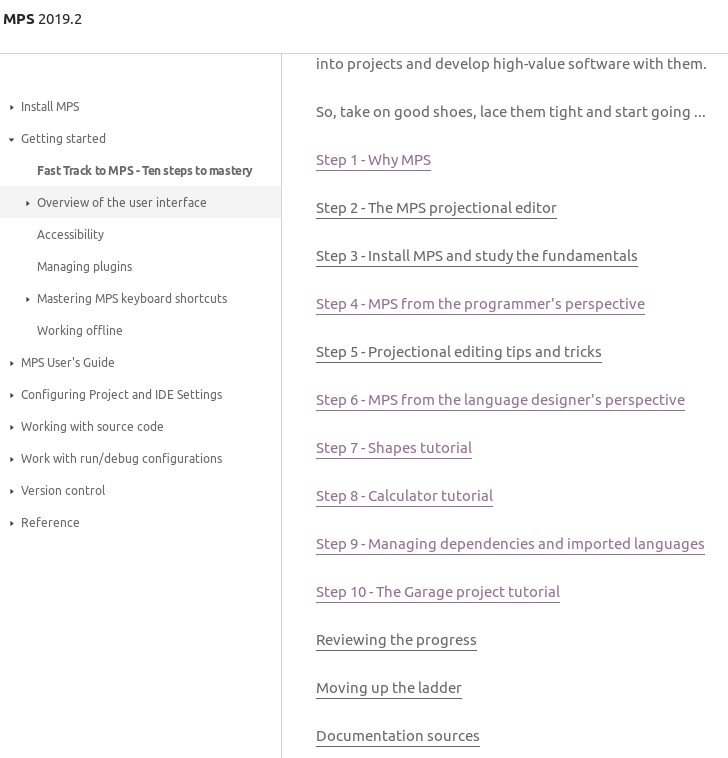
\includegraphics[width=0.7\textwidth]{chapters/fundamentacao/imagens/fastrack.jpg}}

\par\medskip\textbf{Fonte:} \textit{JetBrains} (2019). \par\medskip
\end{figure}


\begin{figure}[h!]
\centering

\caption{\textmd{JetBrains treinamento online gratuito}}
\label{fig:onlinetraining}
\fcolorbox{gray}{white}{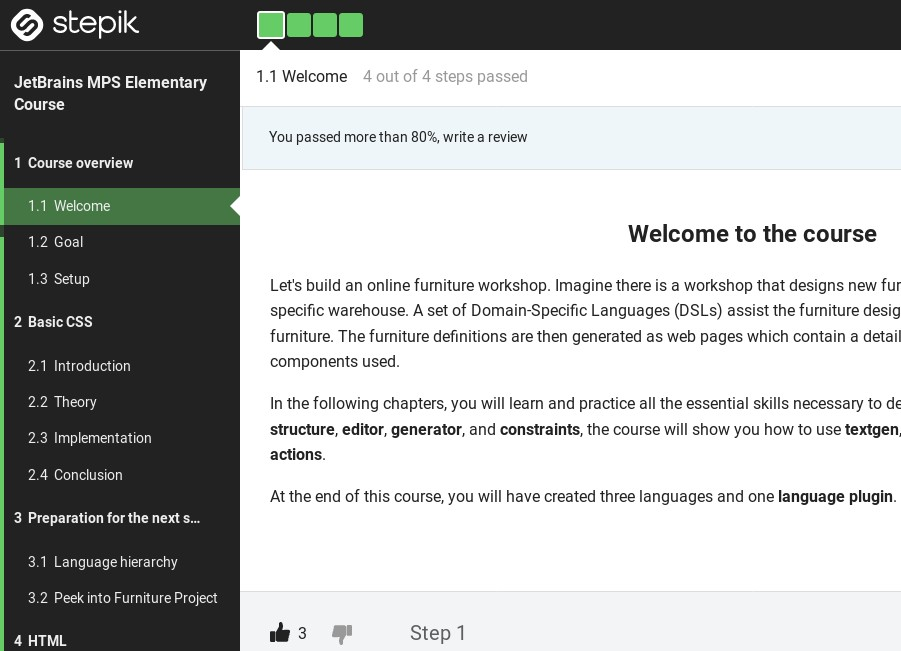
\includegraphics[width=0.7\textwidth]{chapters/fundamentacao/imagens/onlinetraining.jpg}}

\par\medskip\textbf{Fonte:} \textit{JetBrains} (2019). \par\medskip
\end{figure}


\newpage
Tendo em vista que, a presente pesquisa procura reduzir a demanda para os desenvolvedores com relação às mudanças nas regras do sistema de cotas, é importante que a ferramenta ajude em questões de produtividade e possua boa usabilidade. Uma vez que alterações podem surgir, seja em função de mudanças nos documentos de lei, ou até por questões de entendimento sobre determinado requisito de negócio - exemplos dessas situações foram apresentados anteriormente no Capítulo \ref{chap:historicoversoes}.

Nesse sentido, o texto de  \citeonline{voelter2014generic}, apresenta um levantamento sobre a usabilidade do \gls{MPS}, em que 20 usuários do \gls{MPS} foram questionados sobre: "Eu consigo trabalhar produtivamente com o MPS" e "Foi fácil se acostumar com a programação no MPS". Esta pequisa, segundo ele, mostra que os primeiros resultados foram positivos. 

O resultado dessa pesquisa pode ser visto na Figura \ref{fig:usuariosMPS}. São utilizados 5 (cinco) níveis de escala de concordância às 2 (duas) perguntas. O gráfico da esquerda apresenta que a maioria concorda totalmente ou apenas concorda, sobre a pergunta de trabalho com produtividade, enquanto no gráfico da direita, sobre a facilidade de se acostumar com a \gls{IDE}, a concordância é geral \cite{voelter2014generic}.

\begin{figure}[h!]
\centering

\caption{\textmd{Pesquisa sobre usabilidade do MPS}}
\label{fig:usuariosMPS}
\fcolorbox{gray}{white}{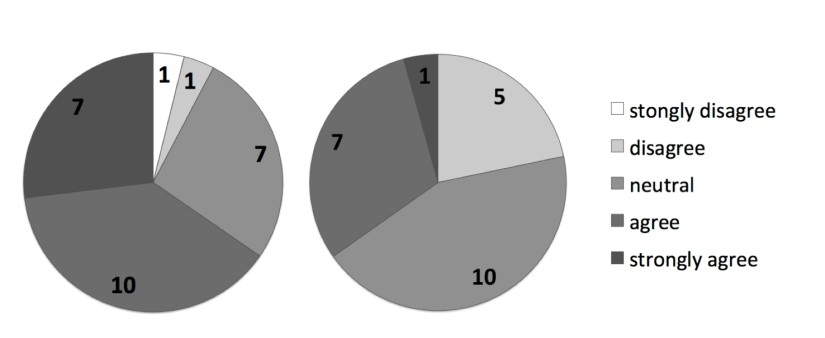
\includegraphics[width=0.9\textwidth]{chapters/fundamentacao/imagens/usuariosMPS.jpg}}

\par\medskip\textbf{Fonte:} \cite{voelter2014generic} \par\medskip
\end{figure}



Segundo \citeonline{volter2011language}, as ferramentas tradicionais baseadas em gramática tornam difícil o desenvolvimento de linguagens, pois possuem limites na composição de gramáticas. Para ele, o \gls{MPS} resolve dois desafios importantes para o desenvolvimento de linguagens: 
\begin{enumerate}
    \item[a)] A composição e mistura de sintaxes diferentes em uma mesma linguagem;
    \item[b)] A modularização e extensão de linguagens.
\end{enumerate}

Esses pontos favorecem o desenvolvimento e reutilização de linguagens, pois no \gls{MPS} é possível criar linguagens novas estendendo definições de outras já existentes, sendo possível combinar conceitos que deveriam ser tratados em diferentes pontos de vista, segregando preocupações da solução, de acordo com as necessidades e preocupações de cada domínio \cite{volter2011language}.

Do ponto de vista do autor da presente pesquisa, o \gls{MPS} se mostra uma ferramenta moderna e madura, sua base de exemplos possui mais de 37 projetos que podem servir como base para facilitar o aprendizado e desenvolvimento de linguagens. É uma ferramenta gratuita com vasta documentação, e por se tratar de uma ferramenta projecional não há a necessidade de manter uma gramática formal ou de desenvolvimento de \textit{parsers}.

Com foco nessa ferramenta e nos conceitos sobre linguagens específicas de domínio apresentados, no Capítulo \ref{chap:proposta} será apresentada a linguagem proposta para ser desenvolvida nessa pesquisa, assim como algumas vantagens que poderão contribuir na geração do código fonte que faz a classificação de candidatos ao sistema de cotas.